\documentclass[acmtog]{acmart}

\usepackage{booktabs} % For formal tables

\usepackage{geometrycollective}


\usepackage[ruled]{algorithm2e} % For algorithms
\renewcommand{\algorithmcfname}{ALGORITHM}
\SetAlFnt{\small}
\SetAlCapFnt{\small}
\SetAlCapNameFnt{\small}
\SetAlCapHSkip{0pt}
\IncMargin{-\parindent}

% Metadata Information
\acmJournal{TOG}
\acmVolume{X}
\acmNumber{X}
\acmArticle{XX}
\acmYear{XXXX}
\acmMonth{-1}

% Copyright
\setcopyright{acmcopyright}
%\setcopyright{acmlicensed}
%\setcopyright{rightsretained}
%\setcopyright{usgov}
%\setcopyright{usgovmixed}
%\setcopyright{cagov}
%\setcopyright{cagovmixed}

% DOI
\acmDOI{XX}

% Paper history
\received{January 20XX}
%\received{March 2009}
%\received[final version]{June 2009}
%\received[accepted]{July 2009}

% \begin{teaserfigure}
%   \centering
%   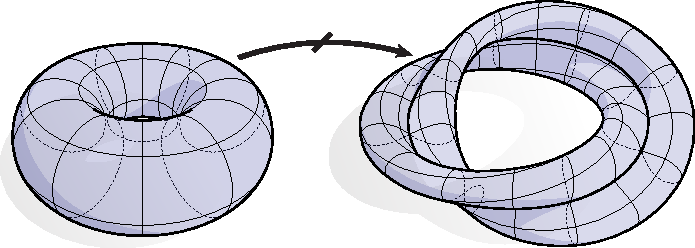
\includegraphics{images/teaser.pdf}
%    \caption{CAPTION.\label{fig:teaser}}
% \end{teaserfigure}

% Document starts
\begin{document}
% Title portion
\title{Circular Arc Triangulations} 
\author{Ethan Lu} 
\author{Keenan Crane} 
\affiliation{%
  \institution{Carnegie Mellon University}
  \streetaddress{5000 Forbes Ave}
  \city{Pittsburgh}
  \state{PA}
  \postcode{15213}}

\renewcommand\shortauthors{Ethan Lu and Keenan Crane}

\begin{abstract}
   This paper explores how triangulations with circular edges can be a valuable primitive for a variety of geometric algorithms.  An extremely common way to discretize smooth surfaces is using Euclidean triangles, with straight edges---however, such triangles do a poor job of capturing some important features of smooth surfaces, such as its curvature (which becomes highly singular), and angle-preserving or \emph{conformal} maps (which cannot preserve angles in the discrete setting).  On the other hand, surface approximations using higher-order patches (NURBS, \etc{}) become difficult to control, and to reason about.  Circular arc triangulations (CATs) provide a middle ground, where only a few additional degrees of freedom give a significant geometric improvement.  We describe a variety of ways of parameterizing CATs, including a novel parameterization by a triangle in a constant-curvature geometry, plus a M\"{o}bius transformation of the plane---different parameterizations in turn allow us to formulate efficient algorithms and optimization problems in various settings.  In particular, we show how to approximate a curved surface by a CAT mesh with curvature only along edges (rather than at vertices); using a connection to \emph{circle patterns} we describe a discrete version of Riemann mapping where angles are directly preserved; and, X.
\end{abstract}


%
% The code below should be generated by the tool at
% http://dl.acm.org/ccs.cfm
% Please copy and paste the code instead of the example below. 
%
\begin{CCSXML}
<ccs2012>
 <concept>
  <concept_id>10010520.10010553.10010562</concept_id>
  <concept_desc>Computer systems organization~Embedded systems</concept_desc>
  <concept_significance>500</concept_significance>
 </concept>
 <concept>
  <concept_id>10010520.10010575.10010755</concept_id>
  <concept_desc>Computer systems organization~Redundancy</concept_desc>
  <concept_significance>300</concept_significance>
 </concept>
 <concept>
  <concept_id>10010520.10010553.10010554</concept_id>
  <concept_desc>Computer systems organization~Robotics</concept_desc>
  <concept_significance>100</concept_significance>
 </concept>
 <concept>
  <concept_id>10003033.10003083.10003095</concept_id>
  <concept_desc>Networks~Network reliability</concept_desc>
  <concept_significance>100</concept_significance>
 </concept>
</ccs2012>  
\end{CCSXML}

\ccsdesc[500]{Computer systems organization~Embedded systems}
\ccsdesc[300]{Computer systems organization~Redundancy}
\ccsdesc{Computer systems organization~Robotics}
\ccsdesc[100]{Networks~Network reliability}

%
% End generated code
%

% We no longer use \terms command
\terms{Design, Algorithms, Performance}

\keywords{Wireless sensor networks, media access control,
multi-channel, radio interference, time synchronization}


\thanks{This work is supported by the National Science Foundation, under grant XXXX, grant XXXX and grant XXXX.}

  % Author's addresses: G. Zhou, Computer Science Department, College of
  % William and Mary; Y. Wu {and} J. A. Stankovic, Computer Science
  % Department, University of Virginia; T. Yan, Eaton Innovation Center;
  % T. He, Computer Science Department, University of Minnesota; C.
  % Huang, Google; T. F. Abdelzaher, (Current address) NASA Ames
  % Research Center, Moffett Field, California 94035.}


\maketitle

\begin{figure}
   \centering
   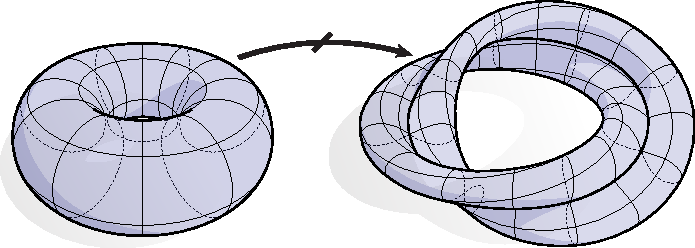
\includegraphics[width=\columnwidth]{images/teaser.pdf}
   \caption{A caption.\label{fig:teaser}}
\end{figure}

Here is a paper.~\cite{reid:scribe}

\begin{tabular}{r|l}
   Column width & \the\columnwidth \\
   Text width & \the\textwidth \\
   Font size & \makeatletter\f@size pt \\
\end{tabular}

% Bibliography
\bibliographystyle{ACM-Reference-Format}
\bibliography{CATs}

\end{document}

%%                         .
%%                        -|-
%%                         |
%%                     .-'~~~`-.
%%                   .'         `.
%%                   |  R  I  P  |
%%                   |           |
%%                   |           |
%%                 \\|           |//
%% ^^^^^^^^^^^^^^^^^^^^^^^^^^^^^^^^^^^^^^^^^^^^^^^^^^^^^
%%                     GRAVEYARD
%% ^^^^^^^^^^^^^^^^^^^^^^^^^^^^^^^^^^^^^^^^^^^^^^^^^^^^^

